\section{Introduction}
\label{introduction}

Since \citet{mcmahan2017communication} propose the \textit{federated average} paradigm, FL has gradually become a promising approach to handle both data privacy and efficient training on the large scale of edged clients, which employs a global server to coordinate local clients jointly train one model. Due to privacy protection, it disables the direct information interaction across clients. All clients must only communicate with an accredited global server. This paradigm creates an unavoidable issue, that is, bandwidth congestion caused by mass communication. Therefore, FL advocates training models on local clients as much as possible within the maximum bandwidth utilization range and only communicates with a part of clients per communication round in a partial participation manner. Under this particular training mechanism, FL needs to effectively split the original problem into several subproblems for local clients to solve in parallel. Because of this harsh limitation, general algorithms are often less efficient in practice. But the \textit{primal dual} methods just match this training pattern, which empowers it with huge application potential and great values in FL.

\textit{Primal dual} methods, which are specified as \textit{Lagrangian primal dual} in this paper, solve the problem by penalizing and relaxing the constraints to the original objective via non-negative Lagrange multipliers, which make great progress in convex optimization. It benefits from the consideration of splitting a large problem into several small simple problems to solve, which has been widely developed and applied in the distributed framework as a global consensus problem. This solution is also well suited to the FL scenarios for its effective split characteristic. Recent studies revealed the application potential of such methods. Since \citet{tran2021feddr} propose the \textit{Randomized Douglas-Rachford Splitting} in FL, which unblocks the study of this important branch. With further exploration of \citet{zhang2021fedpd,durmus2021federated,zhang2021connection}, \textit{federated primal dual} methods are proven to achieve the fast $\mathcal{O}(1/T)$ convergence rate. Then it is expanded to the more complicated scenarios and incorporated with several novel techniques to achieve state-of-the-art~(SOTA) performance in the FL community, which further confirms the great contributions.

\begin{wrapfigure}[16]{r}{0.5\textwidth}
\centering
\vspace{-0.6cm}
    \subfigure[\small Train loss.]{
        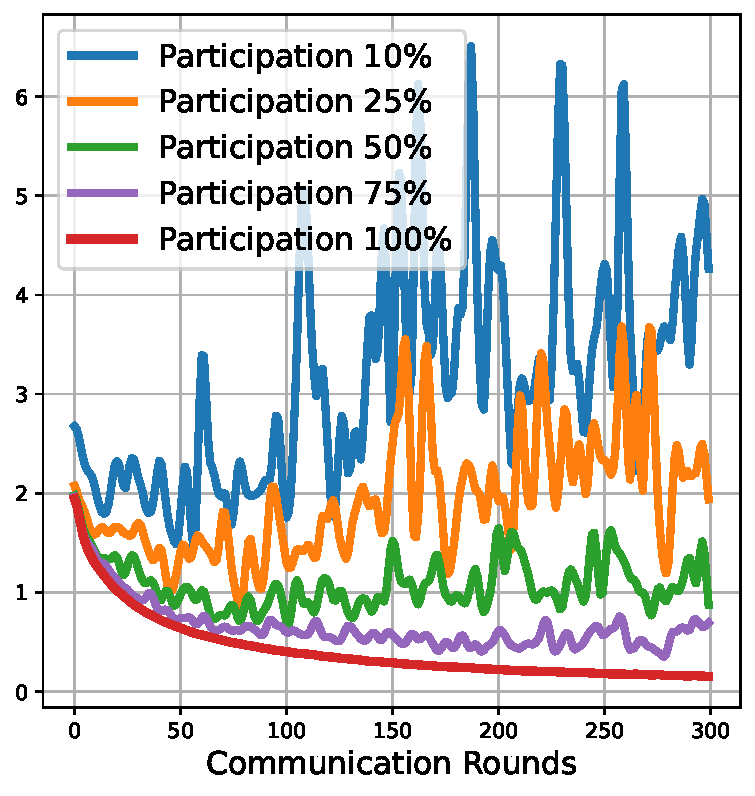
\includegraphics[width=0.24\textwidth]{figure/dual_drift_loss.pdf}}\!\!\!
    \subfigure[\small Test accuracy.]{
	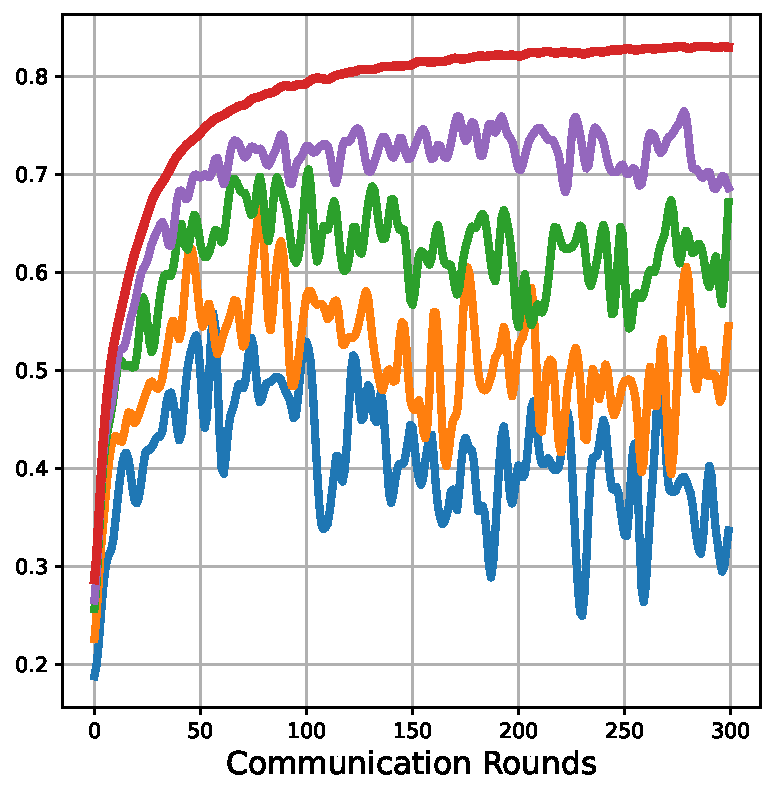
\includegraphics[width=0.245\textwidth]{figure/dual_drift_acc.pdf}}
 \vskip -0.04in
\caption{``\textit{Dual drift}'' issue of the \textit{federated primal dual} method under different participation ratios. When the participation ratio is low, \textit{dual drift} introduces a very large variance, yielding divergence.}
\label{dual drift}
 \vskip -0.1in
\end{wrapfigure}

However, as studies go further, a series of problems of \textit{federated primal dual} methods in the experiments are also exposed. Sensitivity to hyperparameters and fluctuations affected by the large scale makes it extremely unstable in practice, especially in the partial participation manner which is one of the most important concerns in FL. Specifically, \textit{primal dual} methods successfully solve the problems by alternately updating each primal variable and each dual variable. When it is grafted onto the partial participation training in FL, most clients will remain inactive for a long time, which means most of the dual variables will be stagnant and very outdated in the training. As the training process continues, when one long-term inactive client is reactivated to participate in training, the solving process of its local subproblem will become extremely unstable due to excessive differences between the primal and dual variables, and sometimes even fail. We call this a ``\textit{dual drift}'' problem, which is also one of the most formidable challenges in practice in FL. In Fig.\ref{dual drift}, we clearly show how the ``\textit{dual drift}'' deteriorates as the participation ratio decreases. This instability seriously hinders the application of such methods.

To efficiently expand the \textit{primal dual} methods to partial participation scenarios while enhancing the training stability in practice, and further alleviate the ``\textit{dual drift}'' problem, we propose a novel algorithm, named \textit{\textbf{A}ligned \textbf{Fed}erated \textbf{P}rimal \textbf{D}ual}~(\textit{\textbf{A-FedPD}}), which constructs the virtual dual updates for those unparticipated clients per communication round to align with primal variables. Concretely, after each communication round, we first aggregate the local solutions received from active clients as the unbiased approximation of the local solution of those unparticipated clients. Then we provide a virtual update on the dual variables to align with the primal variable in the training. Updating errors for dual variables will be diminished as global consensus is achieved. The proposed \textit{A-FedPD} method enables unparticipated clients to keep up-to-date, which approximates the quasi-full-participation training, which can efficiently alleviate the ``\textit{dual drift}'' in practice.

Furthermore, we provide a comprehensive analysis of the optimization and generalization efficiency of the proposed \textit{A-FedPD} method, which also could be easily extended to the whole \textit{federated primal dual family}. On smooth non-convex objectives, compared with the vanilla \textit{FedAvg} method, the \textit{A-FedPD} could achieve a fast $\mathcal{O}(1/T)$ convergence rate which maintains consistent with SOTA \textit{federated primal dual} methods. Moreover, it could support longer local training without affecting stability. Under the same training costs, the \textit{A-FedPD} method achieves less generalization error. We conduct extensive experiments to validate its efficiency across several general federated setups. We also test a simple variant to show its good scalability incorporated with other novel techniques in FL.

We summarize our major contributions as follows:
\begin{itemize}
    \item We review the development of \textit{federated primal dual family} and point out one of its most formidable challenges in the practical application in FL, which is summarized as the ``\textit{dual drift}'' problem in this paper.
    \item We propose a novel \textit{A-FedPD} method to alleviate the ``\textit{dual drift}'', which constructs the virtual update for dual variables of those unparticipated clients to align with primal variables.
    \item We provide a comprehensive analysis of the optimization and generalization efficiency of \textit{A-FedPD}. It could achieve a fast convergence rate and a lower generalization error bound than the vanilla \textit{FedAvg} method.
    \item Extensive experiments are conducted to validate the performance of the \textit{A-FedPD} method. Furthermore, we test a simple variant of it to show its good scalability.
\end{itemize}



